\documentclass[letterpaper,11pt]{article}
\usepackage[dvips]{graphicx}
\usepackage{epsfig}
\usepackage{url}
\usepackage{palatino}
\usepackage{geometry}

\raggedbottom
%\topmargin=-.9cm
%\topskip=-3.5cm
%\textheight=24.5cm
%\textwidth=16.8cm
%\oddsidemargin=-0.5cm
%\evensidemargin=-0.5cm 
\parindent=0mm
\topsep=0.5ex
\itemsep=0.5ex
\geometry{tmargin=3.5cm, lmargin=3.0cm, rmargin=3.0cm, bmargin=1.0cm}

\makeatletter

\newcommand\subsubsubsection{\@startsection {paragraph}{1}{\z@}%
                                   {-3.5ex \@plus -1ex \@minus -.2ex}%
                                   {1.5ex \@plus.2ex}%
                                   {\normalfont\bfseries}}
%\makeatother

%\def\thebibliography#1{\section*{}\list
% {[\arabic{enumi}]}{\settowidth\labelwidth{[#1]}\leftmargin\labelwidth
% \advance\leftmargin\labelsep
% \usecounter{enumi}}
% \def\newblock{\hskip .11em plus .33em minus .07em}
% \sloppy\clubpenalty4000\widowpenalty4000
% \sfcode`\.=1000\relax}
%\let\endthebibliography=\endlist

\def\contentsname{Table of Contents}
%\def\listfigurename{List of Figuras}

%\input{psfig}

\newcommand\Observatory{Atama Large Millimiter/submillimiter Array}
\newcommand\Title{Alma Common Software Component Code Generation}
\newcommand\Subtitle{Alma Common Software}
\newcommand\Type{Project Documentation}
\newcommand\Version{B}
\newcommand\Document{ALMA-BBB-CCC-A-DDD}
\newcommand\PreparedA{Alexis Tejeda}
\newcommand\PDate{2010-04-23 }
\newcommand\Approved{}
\newcommand\Released{}
\newcommand\Keywords{Alma Common Software Component Java Code Generator}
\newcommand\Department{JAO Computing Group}
\newcommand\Date{2010-31-01}
\newcommand\Status{Draft}
\newcommand{\smartmonitor}{{\bf SmartMonitor} }
\newcommand{\control}{{\tt CONTROL} }

\begin{document}
\pagenumbering{roman}

\pagestyle{empty}


%\begin{picture}(0,0)
%\vadjust{\vskip 1 cm}
%\centerline{

%\special{ps: plotfile /vlt/templates/forLaTeX/pbvlt.000}}
%\medskip
%\vadjust{\vskip 1 cm}
%\end{picture}

%\begin{center}
%\bf
%\Large
%\hspace{-1.0cm} {\Large{E U R O P E A N\hspace{0.5cm}S O U T H E R N\hspace{0.5cm} O B S E R V A T O R Y}\\%
%\small{Organisation Europ\'{e}enne pour des Recherches Astronomiques dans 
%l'H\'{e}misph\`{e} Austral}\\%
%\small{Europ\"{a}ische Organisation f\"{u}r astronomische Forschung in der
% s\"{u}dlichen Hemisph\"{a}re}}
\begin{center}%
%    \begin{tabular}{ll}
%    \hspace{-1.5cm}
%    
\epsfig{file=images/alma_logo}

\vspace{-1.5cm}
\begin{figure*}[h!t]
\begin{center}
\includegraphics*[scale=0.8]{images/alma_logo}
\end{center}
\end{figure*}
\vspace{1cm}

%    &
%  %  \hspace{0.2cm}
%\vspace{-5cm}
%    \begin{tabular}{l}
%      \Large{E U R O P E A N\hspace{0.5cm} S O U T H E R N\hspace{0.5cm} O B S E
% R V A T O R Y}\bigskip\\%
%      \small{Organisation Europ\'{e}enne pour des Recherches Astronomiques dans 
%l'H\'{e}misph\`{e} Austral}\bigskip\\
%      \small{Europ\"{a}ische Organisation f\"{u}r astronomische Forschung in der
% s\"{u}dlichen Hemisph\"{a}re}
% %     \hspace{8.0cm}
%\vspace{5cm}
%    \end{tabular}
%  \end{tabular}
%
%\vspace{-2.4cm}
%\Huge
%\hspace{-1.7cm} {\Observatory}
%\vspace{2.6cm}

\begin{picture}(10,1)(0,0)
\put(-190,0){\line(0,-1){6}}
\put(-190,0){\line(1,0){6}}
\put(190,0){\line(0,-1){6}}
\put(184,0){\line(1,0){6}}
\end{picture}

% ***********************************************************************************
% DOCUMENT IDENTIFICATION SECTION
%
% Document Title, Up to four lines. The first or the last should be the
% document type (e.g., Statement of Work, Functional Specification, etc.)
% 

\large
%\hspace{-1.7cm} {\bf \Department }             % <<<<<<< update (if needed)
%
%\hspace{-1.7cm} {\bf -- }                      % <<<<<<< available extra line (for long title)

\vspace{0.5cm}
\hspace{-0.5cm} {\bf \Large \Title }     
             % <<<<<<< subject
%\begin{center}
%{\bf \Subtitle }   
%\end{center}  % <<<<<<< f.i., Functional Specification, User Manual, etc. 

\begin{center} 
{\bf \Type }  
\end{center}  

\normalsize
\vspace{0.5cm}

\hspace{-0.5cm} { \Document }          % <<<<<<< Document number 
\vspace{0.5cm}

\hspace{-0.5cm} {Version: \Version}                 % <<<<<<< Version [/preparation]
\vspace{0.1cm}

\hspace{-0.5cm} {Status: \Status }          % <<<<<<< Status
\vspace{0.5cm}

\hspace{-0.5cm} { \Date }                  % <<<<<<< Date 
\vspace{0.5cm}

\begin{picture}(10,1)(0,0)
\put(-196,0){\line(0,1){6}}
\put(-196,0){\line(1,0){6}}
\put(196,0){\line(0,1){6}}
\put(190,0){\line(1,0){6}}
\end{picture}

% **************
%  WARNING NOTICE FOR PRELIMINARY VERSION ISSUED FOR REVIEW AND NOT ARCHIVED
%
% <<<<<<<< Comment the following in the final version

%\vspace{1.0cm}
%\begin{center}
%\LARGE
%{\bf Prepared for Review}
%\end{center}
%\vspace{1.6cm}

% <<<<<<<< Uncomment the following in the final version (ARCHIVE)
%\vspace{3.6cm}
\vspace{2.5cm}

%
% ***********************************************************************************
% SIGNATURE SECTION
%
%   - AUTHOR
%

\vspace{-1.5cm}
\begin{center}
\normalsize
{\bf Keywords: \Keywords}
%\vspace{0.5cm}
\end{center}
\vspace{0.5cm}

%{\small {\tt \hspace{-1cm}{\Prepared} \hspace{0.8cm}{\PDate }}}  % <<<<<<< Author name and Date
{\small {\tt \hspace{-0.8cm}{\PreparedA} \hspace{2.2cm}{\PDate }}}  % <<<<<<<Author name and Date
\vspace{-0.3cm}

\large
\hspace{-0.7cm} {Prepared  \small . . . . . . . . . . . . . . . . . . . . . . . . . . . . . . . . . . . . . . . . . . . . . . . . . . . . . . .}

\footnotesize
\hspace{2.5cm}{Name} \hspace{4cm}{Date}  \hspace{2cm}{Signature}
\vspace{1cm}

%{\small {\tt \hspace{-1cm}{\Prepared} \hspace{0.8cm}{\PDate }}}  % <<<<<<< Author name and Date
%{\small {\tt \hspace{0.5cm}{\Prepared} \hspace{3cm}{\PDate }}}  % <<<<<<< Author name and Date

\vspace{-0.3cm}


%   - APPROVER

\normalsize
{\small {\tt \hspace{-5.5cm}{\Approved}}}     % <<<<<<< approver name
\vspace{-0.3cm}

\large
\hspace{-0.7cm} {Approved  \small . . . . . . . . . . . . . . . . . . . . . . . . . . . . . . . . . . . . . . . . . . . . . . . . . . . . . . .}

\footnotesize
\hspace{2.5cm}{Name} \hspace{4cm}{Date} \hspace{2cm}{Signature}
\vspace{1cm}

%   - RELEASER

\normalsize
{\small {\tt \hspace{-5.5cm}{\Released}}}  %  <<<<<<< releaser name
\vspace{-0.3cm}

\large
\hspace{-0.7cm} {Released  \small . . . . . . . . . . . . . . . . . . . . . . . . . . . . . . . . . . . . . . . . . . . . . . . . . . . . . . .}

\footnotesize
\hspace{2.5cm}{Name} \hspace{4cm}{Date} \hspace{2cm}{Signature}
\end{center}

% ***********************************************************************************
% PAGE HEADING SECTION
%
\clearpage
\pagestyle{myheadings}
\markboth
{\underline{ \Title - \Version \hspace*{2.5cm} \Document}}   %  <<<<<<<
%comment for single side document 
{\underline{ \Title - \Version \hspace*{2.5cm} }}   %

 %  <<<<<<< comment for single side document
%{\underline{ \Title - \Version \hspace*{2.5cm} \Document}}   %  <<<<<<<
%comment for single side document
% {}                                                                                   %  <<<<<<< uncomment for single side document
% {\underline{ Document Title - n.m[/prep.k] \hspace*{2.5cm} VLT-xxxx-ESO-ccccc-nnnn}} %  <<<<<<< uncomment for single side document
% <<<<<<<< comment the following in the case of a single side document 
%\vspace*{8 cm}
%\begin{center}
%This page was intentionally left blank
%\end{center}
%\newpage


% ***********************************************************************************
% CHANGE RECORD SECTION
%
\normalsize
\begin{center}
{\bf Change Record}
\vskip 0.5 cm
\begin{tabular}{|c|c|l|l|}   
\hline& & & \\
Issue/Rev. & Date &  Section/Parag. affected &
 Reason/Initiation/Documents/Remarks  \\
& & &  \\     \hline
%            &            &          &              \\
%n.m[/prep.k]& dd/mm/yy   & .....    &  .........   \\   %  <<<<<<< (prep. record shall be deleted in the final edition)
            &            &          &              \\
 A          & 2010-02-10 & All      &  Creation, A.TEJEDA.   \\
            & & &  \\     \hline
            &            &          &              \\
 B          & 2010-04-23 & All      &  Update all document, ATEJEDA.   \\
            &            &          &              \\
\hline
\end{tabular}
\end{center}
\normalsize

% <<<<<<<< comment the following in the case of a single side document 
%\newpage
%\vspace*{8 cm}
%\begin{center}
%This page was intentionally left blank
%\end{center}

% ***********************************************************************************
% INDEX SECTION   (INDEX IS MANDATORY FOR DOCUMENTS OF MORE THAN 6 PAGES
%
\newpage

\tableofcontents
\listoffigures         %  <<<<<<< optional

% <<<<<<<< comment the following in the case of a double side document and 
%          an even number of index pages.
\newpage
%\vspace*{8 cm}
%\begin{center}
%This page was intentionally left blank
%\end{center}
%\pagebreak

% ***********************************************************************************
% BEGINNING OF TEXT 
%
\parskip=2mm
\pagenumbering{arabic}
\setcounter{page}{1}

%% INTRODUCTION
��W]o�0}ﯰ�kkH�T��j���>Gp����qBx�o�t���I�ZJ$��9���=���M�КȔ
>3F�2�(g����c��/�
��J��~��ۧ�)�ܚf�e��)(!1�+��/0�2��B�(��U�����J�!&3��%�b�����|��Dk`3�rYì`���B�I/�Ж�{
tBd6NDJu�ʓN���'��Ju��&�咪��o��$*R���ڰR�1v���vךN��WM���>��}.��\:�.!������/Y�\��yR�>b��:#�%UJX�X�������؛J쿸����*Zl>H�=� �5M��H��)W���|{w��]�~�i(��!p�M���!\р��Y3f)���C����*L9�2낂ANd�P�4�6��8|EׯO;���U��#��T�=��Q7!�����m5�j��t!�ȕ��L]Y��n�-C���z��CFJ���㫃���ߜ�E������S6CQC��֏)�q��\�a���FصctY�l��1��cX���ұ���Ȧ�R�,�b��(�F\�w�!��K����IK3�K�)�Cn.���Σ%Ĕ�z��S�*�V
}��W�&���[Ў_A�����<t��<�f�黴��W#<u�󘚮���Ų�#�=_�cҿ������g�}�3�fm����@wMi~�p����
\section{PROJECT OVERVIEW}
\subsection{Previous Work}
The work done before this project is related to the thesis$[1]$ of Nicolas
Troncoso, which gives the very beginning to the ACS Code Generation based on UML
metamodels, this project will cover and continue the work already done
, proposed in the thesis as a 'Future Work', like the implementation of
inheritance, more complex models, separation of implemented and generated
classes and have a full implemented code generator for ACS.

\subsection{Project Objectives}
The main goal/objective in the project is have a full Standalone Java Component
Code Generator for Alma Common Software under Eclipse Modeling Framework
umbrella, this, is divided in specific objectives:

\begin{itemize}
\item Project based in Open Architecture Ware 5:\\
All the project has to be based on Open Architecture Ware 5, now under the EMF
umbrella.
 
\item Managment of complex UML Models:\\
In complex UML models, the use of stereotypes that allow to filter the models
to generate, this mean that a class will have a stereotype to identify if this
class will be generated or not, this is for not re-write classes already
generated. This objective is considered a critical factor for the success of
the project.

\item Alma Common Software - Notification Channels Support:\\ 
A full code generation support for ACS Notification Channels, generate all
necessary code from a UML model that represents the association between the
Supplier and Consumers, the generator must be able to generate the
ready-to-implement code for Notification Channels. This objective is
considered a critical factor for the success of the project.

\item Standalone Code Generator: \\
The development of the generator should be under the EMF, however one of the
critical requirements is have the generator as Standalone, this means that the
generator have to work outside the Eclipse IDE dinamicly with any UML
model/metamodel specified by command line. The generator have to generate all
the classes, plus empty skelletons for the user implementation. or regenerate
only the basic classes, this mean only generates the templates for user
modification. This objective is considered a critical factor for the success
of the project.

\item The generated code must be Java:\\ 
At first, all the code generated must be in Java, later, if the time allow,
then implement the code generator templates for C++ and Python, it's more
importante in this project have a full support Java for the code generated
than a semi-implementation of all programming languages.

\item Separation between the generated classes and implemented classes:\\
Complete the separation between the generated classes and the implemented
classes, this mean the code generator has to know how to separate the
implemented classes and the already generated classesfor the code generation
for not overwriting.

\item Inheritance implementation:\\
Actually, the implementation in the generator of model-inheritance is not fully
supported, the developers should define how implement this model behavior in
the code generator without affect all work already done.
\end{itemize}

\subsection{Project Scope}
The project scope cover the development of the Code Generator for ACS,
initially the project will only generate the Java code implementation from a
UML model under the XMI2.0 standard, in which, there are three importants
points defined as critical and project milestones.

\begin{itemize}
	\item Standalone Java Component Code Generator.
	\item Notification Channels and Inheritance Support for UML models.
	\item Code Generator based on Open Architecture Ware 5.
\end{itemize}
Each one of this points are explained more consistently in Goals and Objectives
sections in this document.

\subsection{Roles and Responsibilities}
\begin{itemize}
\item AlexisTejeda (UCN) Deployment Manager, Requirements Reviewer, Architecture
Reviewer, Configuration Manager, Change Control Manager . 
\item GabrielZamora (UTFSM) Deployment Manager, Requirements Reviewer, Architecture Reviewer, Configuration Manager, Change Control Manager.
\item GianlucaChiozzi (ESO) Client, End User, Requirements Reviewer, Change Control Manager.
\item JorgeIbsen (ESO / JAO Computing Manager)Project Manager, Requirements Reviewer.
\item NicolasTroncoso (JAO/AUI) Project Manager, Requirements Reviewer, Architecture Reviewer. 
\end{itemize}

\newpage










\section{DESIGN OVERVIEW}
\subsection{EMF - Open Architecture Ware 5}
The component code generator for Alma Common Software initially created before,
was supported on Open Architecture Ware 4, since is a requirement have the
code generator based on Open Architecture Ware 5, the previous work was
migrated to oaW 5, this means that the code generator is based now on Eclipse
Modeling Framework (EMF), mainly in Xtend and Xpand subprojects.\\
\\
EMF supports many types of models like Ecore (EMF native models), UML2 models,
or, in this case meta-metamodels in XMI2.0 format. Actually the generator
support a XMI2.0 meta-metamodels, mostly of this models are created and exported
from MagicDraw UML Diagram Tool, this program generate the necessary XMI files
for later generate the code component to be implemented. 
Is important to specify that the models need a profile file, which defines the
stereotypes for use in the generator, where they differentiate the
characteristics of UML model.

\subsubsection{Stereotypes}
In UML models, the use of stereotypes helps to distinguish the classes that
must be generated and how must be generated. This stereotypes are defined in
the UML profile file, which is created when the UML model is exported from
MagicDraw.\\
One of each classes must have a stereotype defined to know how the code must be
generated, i.e.: 

\begin{figure*}[h!t]
\begin{center}
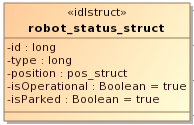
\includegraphics[scale=0.3]{images/idlstruct}
\caption{\label{fig:ex_diag}Example class with a stereotype}
\end{center}
\end{figure*}

The class robot status struct has the \verb+<<IDLStruct>>+ stereotype, then the
generator call the IDLStruct template and generate the code of an IDL file of ACS.\\
Full detail and description of the stereotypes used in this project, please
refer to the Quick How To section in this document.\\
\\
Exist three types of stereotypes, see 'Quick Reference User Manual' for full
description of each stereotype:
\begin{itemize}
	\item Class stereotype : applies to classes like \verb+<<IDLStruct>>+
	stereotype.
	\item Property stereotype : applies to class level variables. 
	\item Operation stereotype : applies to a method of a class.
\end{itemize}


\subsubsection{Xtend/Xpand}
Since owA was migrated to EMF, the code generator is based on a mixture of EMF
subprojects(Xpand/Xtend/Xtext) , the EMF subprojects which are used, are:

\begin{itemize}
	\item Xtend : provides the possibility to define rich libraries of independent
	operations and non-invasive metamodel extensions based on either Java methods
	or oAW expressions. Those libraries can be referenced from all other textual
	languages, that are based on the expressions framework, in this case Xpand.
	\item Xpand : A programming language which allow to define the templates of
	the generator and controll the output generation.
\end{itemize}

\subsubsection{Workflow File Configuration}
The workflow, is a EMF XML configuration file that controll the workflow of the
generator, in which, where configured the paths of UML expoted models,
output folder, templates used, code beautifiers and the package name
definition for the generated code.\\
\\
The path of the model to generate, the generated code output folder path and
the UML profile file path are specified using dynamic workflow propertys by
\$\{myVariable\} sintax. These properties can be configured dynamically in the
Java program (using String Hashmap) that call the generator, or by command
line.\\
\\
Also the templates to use in the generation are specified in the configuration
file as 'Workflow Components'.\\
\\
The components must have defined :
\begin{itemize}
	\item Output path : the output path for the generated file, this is specified
	by a global property in the workflow configuration as \$\{ouputFolderURI\} 
	property.
	\item UML profile : this is specified by a global property in the workflow
	configuration as \$\{profileFileURI\} property, the generator only support
	maximum three profile files.
	\item Template : the template to use.
	\item Beautifiers : XML or Java code beautifiers.
	\item VetoStrategy : only is specified if the component will use a Veto
	Strategy, see 'Generator Optimization' section for more info about this.
	\item File encoding : by default UTF-8.
\end{itemize}

An example configuration for a component, in this case a java class files
component generator :
\begin{center}
\begin{verbatim}
    <component id="genjava" class="org.eclipse.xpand2.Generator"
     skipOnErrors="true"> 
    <fileEncoding value="UTF-8" />
        <metaModel idRef="default_profile"/>
        <expand value="templates::java::JavaRoot::Root FOR model"/>
        <outlet path="${ouputFolderURI}">
            <vetoStrategy
             class="cl.alma.acs.ccg.vetostrategy.ACSCCGVetoStrategy" /> 
            <postprocessor 
             class="org.eclipse.xpand2.output.JavaBeautifier"/>
        </outlet>
        <prSrcPaths value="${ouputFolderURI}"/>
    </component> 
\end{verbatim}
\end{center}

In the project, exists three workflow files, a Java, C++ and Python. Python
and C++ workflow files are ready to be implemented, only Java workflow is full
implemented for the generator.\\
\\
The workflow file is based in oaW 5, this means that the file presents many
changes from his previous version, more info about the migration of the
workflow, see 'oaW 4 to oaW 5 Migration How To' section in this document. 

\subsubsection{Template Files}
Template files controll the output code generation. Each class in the UML model
is analyzed by the template file, the template check the stereotype of the
class and generate the output file. The templates are based in the Xpand
programming language [4].\\
All templates are encoded in UTF-8 by the use of 'guillimets' [4].

\subsubsection{Xtend Util Helper}
In the generator templates folder exists a Xtend file, this file is a helper
for the templates files, in which, are defined helper functions like if a class
is inherited from other class. More info about the functions, see 'Quick
Reference User Manual' in this document.


\subsection{Generator Optimization}
With a simple model (20 classes) the generator can take about 8 or 10 seconds
to generate the code in a Dual CPU@1.73GHz with 2048 MB RAM, but, if the model
is more complex, then the generation can take longer, this is no problem at
all, the problem comes when the code must be generated again for any
reason, like add a method in a class or add another class in the model. This is
a problem, because, every time we want re-generate the code, will take the same
time as the first generation even if there are no changes in the model (same
code to generate.)\\
\\
To fix this, the use of EMF Veto Strategy is implemented in the components
workflow file configuration. This strategy is class that implements a EMF Veto
interface class, in which each file to be generated, is analyzed if presents any
changes, if there any changes, the files is generated again, if not, the file
is not generated again.\\
\\
This strategy improves the generation time in regeneration, complex models,
and model refactoring.
%\begin{center}
%TABLE OF TIMES
%\end{center}
\section{COMPONENT CODE GENERATOR FEATURES}

In this section will be describe the main features of the code generator, such
as the inheritance, notification channels, a standalone generator, code
regeneration strategies.

\subsection{A Stand-alone Generator}
The component code generator was designed to be a standalone application,
this means, can be executed in any O.S. as a Java Program, JAR Package or
Eclipse Plugin outside of EMF or Eclipse EMF project.\\
\\
The generator supports three ways to be a standalone :
\begin{itemize}
  \item JAR Package : The binary files are packaged in a JAR Java file using
  Ant or Eclipse Ant.
  \item Eclipse Plugin : A simple Eclipse plugin as a Jar file.
  \item Command Line : A Java command line program.
\end{itemize}
Also, the generator contains all the packages to be executed without EMF and 
can be imported to other environments running Java.

All the binarys can be dowloaded, for this, see the `Project Paths` in this
document.

\subsection{Basic Component Modeling}

The basic component model contains a at least a Container and a Component
class also a IDL struct or enumeration class.

\begin{figure*}[h!t]
\begin{center}
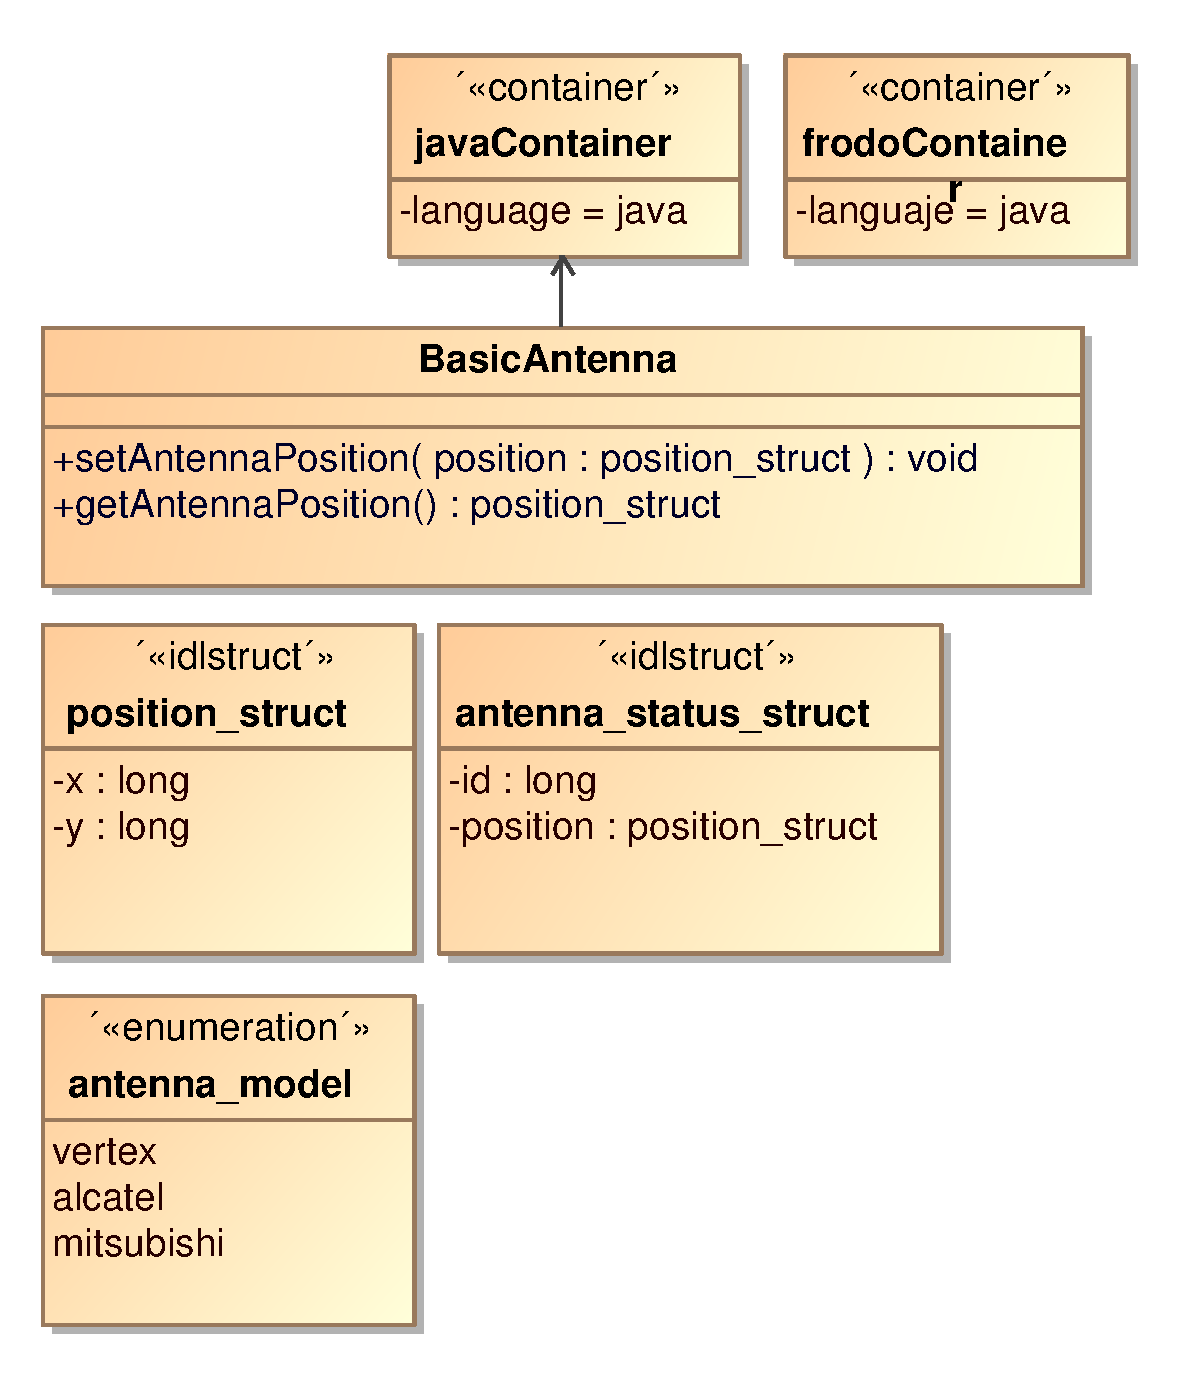
\includegraphics[scale=0.36]{images/example1}
\caption{\label{fig:vs_diag}Basic Model Definition}
\end{center}
\end{figure*} 

This example can be downloaded from:
http://acsccg.googlecode.com/files/example1.tar.gz

\subsubsection{Container Definition}
Every model should have defined at least one container. This is defined by the
stereotype  \verb+<<container>>+ and the class must have defined a property
called  `language`, the value of this property is the programming language that
the container will support (cpp, java, python).
All the containers defined are generated in the CDB configuration in the
generated code.

\begin{figure*}[h!t]
\begin{center}
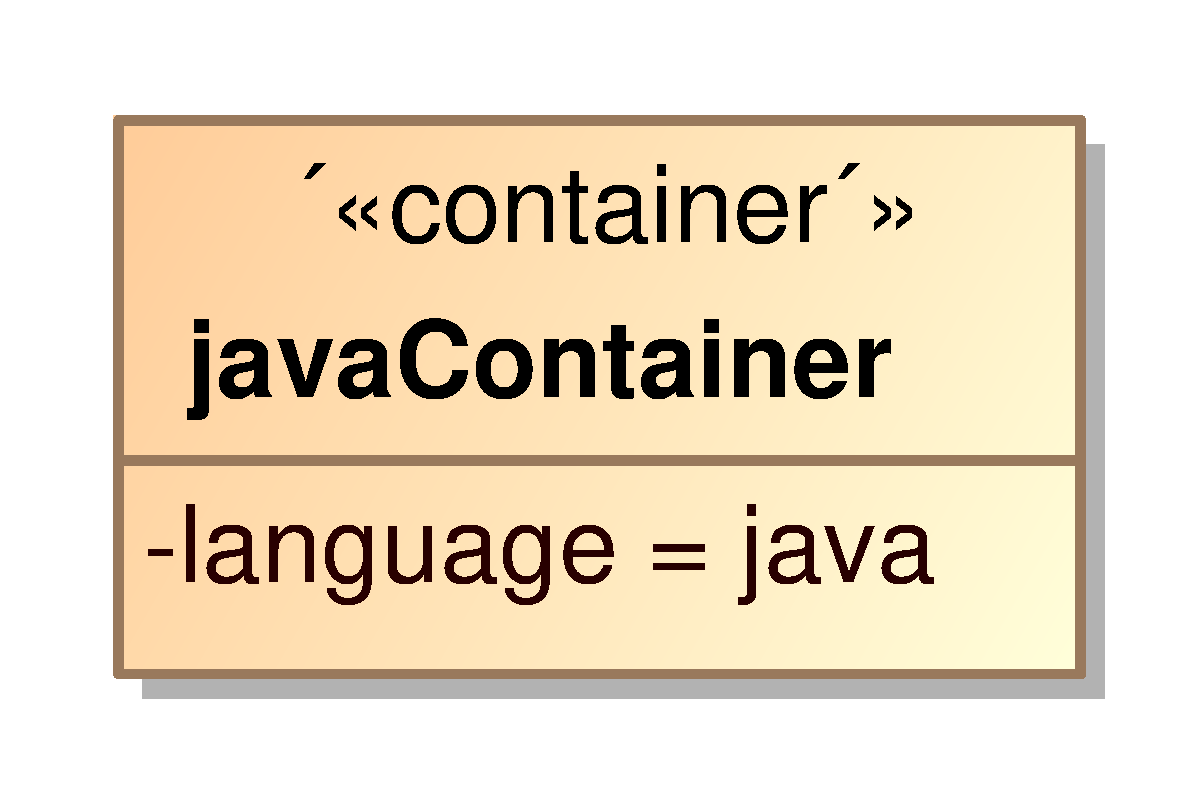
\includegraphics[scale=0.18]{images/container}
\caption{\label{fig:vs_diag}Container Definition}
\end{center}
\end{figure*} 

In the example above, the class \verb+javaContainer+ has the stereotype
\verb+<<container>>+ and the languaje for this container is \verb+java+.
Below, is the code generated for the containers, in this case the
\verb+javaContainer+.
\begin{center}
\begin{verbatim}
test/
`-- CDB
    `-- MACI
        |-- Components
        |   `-- Components.xml
        |-- Containers
        |   `-- javaContainer
        |       `-- javaContainer.xml
        `-- Managers
            `-- Manager
                `-- Manager.xml
\end{verbatim}
\end{center}

And the \verb+javaContainer.xml+ code:
\begin{center}
\begin{verbatim}
<?xml version="1.0" encoding="ISO-8859-1"?>
<Container 
    xmlns:xsi="http://www.w3.org/2001/XMLSchema-instance" 
    xmlns="urn:schemas-cosylab-com:Container:1.0" 
    xmlns:log="urn:schemas-cosylab-com:LoggingConfig:1.0" 
    ImplLang="java"
    >
    <Autoload>
     </Autoload>
     <LoggingConfig>
        <log:_ Name="jacorb@javaContainer" 
        minLogLevel="5" 
        minLogLevelLocal="5"/>
    </LoggingConfig>
</Container>
\end{verbatim}
\end{center}

\subsubsection{Component Definition}
Every class without a stereotype, the generator will recognize the class as a
component. Every class must be related to a container class, if the class is not
related to a container, the generator will not config the component in the CDB.
All component classes that are related to a container the generator will
generate:
\begin{itemize}
	\item The source component Java code (with his methods).
	\item The source java helper class.
	\item The IDL interface (with component methods).
	\item The CDB configuration for the component.
	\item The Makefile is generated with all IDL interfaces which represents each
	class component in the model.
\end{itemize}

 \begin{figure*}[h!t]
\begin{center}
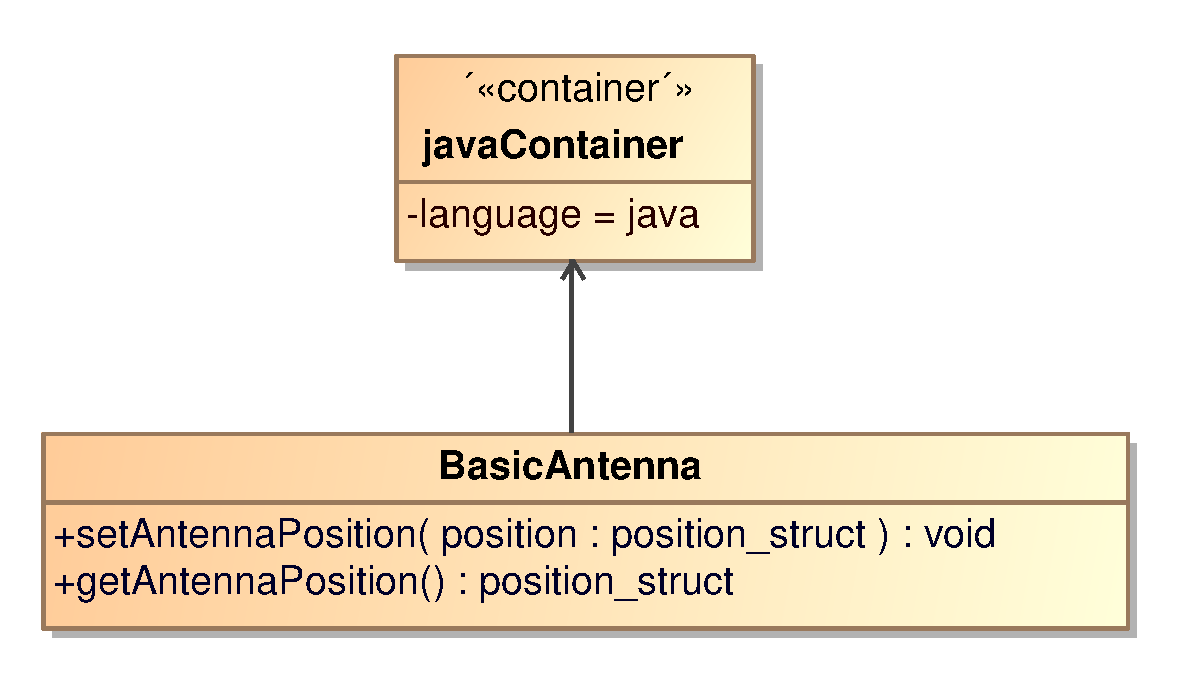
\includegraphics[scale=0.4]{images/basiccomponent}
\caption{\label{fig:vs_diag}Basic Component Definition}
\end{center}
\end{figure*} 

In the example above the class  \verb+BasicAntenna+ is a ACS component and is
related to the  \verb+javaContainer+ the name of the Java classes are prefixed
by `Base` also the IDL interfaces generated are prefixed by `Base` and example
of this the \verb+BasicAntenna+ class is generated as
\verb+BasicAntennaBase.java+ class.

\subsubsection{IDL Structs Definition}

The IDL structs are defined in a class with the stereotype \verb+<<idlstruct>>+.
In the example below the class \verb+<<antenna_status_struct>>+ has two property
that the generator will implement.

\begin{figure*}[h!t]
\begin{center}
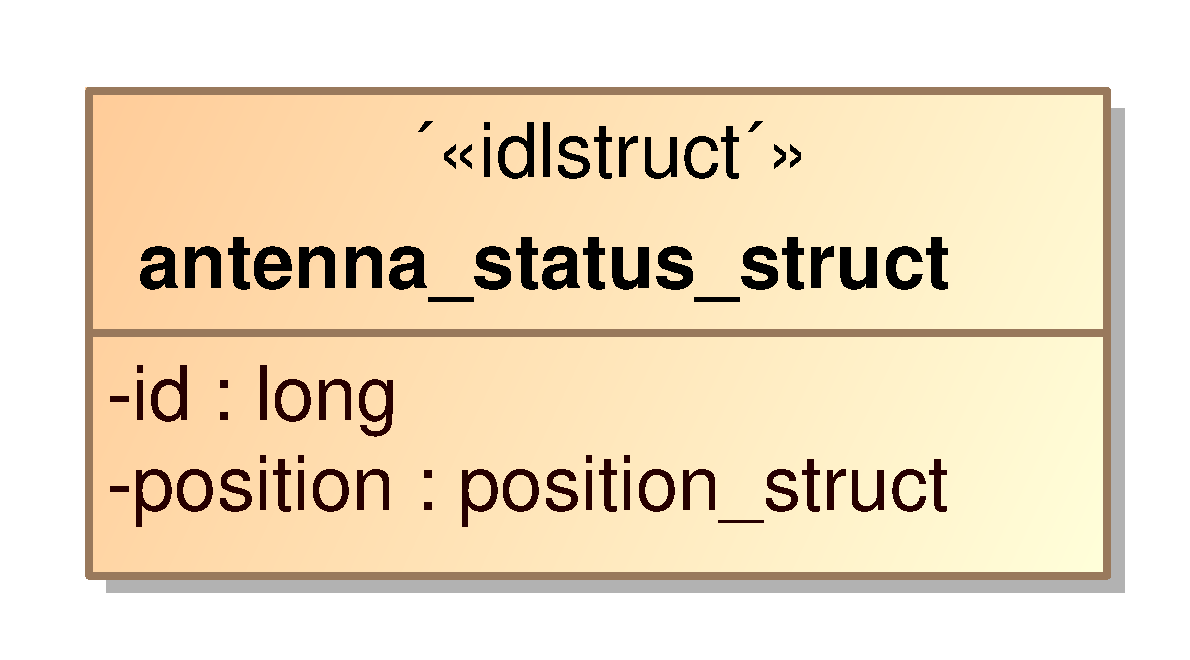
\includegraphics[scale=0.2]{images/idlstructb}
\caption{\label{fig:vs_diag}IDL Struct Definition}
\end{center}
\end{figure*} 

The code generated for that struct is defined in a common IDL interface, this
IDL file has the name of the project, in this case \verb+example1Common.idl+,
an example of the code generated:

\begin{center}
\begin{verbatim}
#ifndef example3_IDL
#define example3_IDL
#pragma prefix "alma"

module example3
{
    struct position_struct {
        long x;
        long y;
    };
    typedef sequence<position_struct> position_struct_seq;
	
    struct antenna_status_struct {
        long id;
        position_struct position;
    };
    typedef sequence<antenna_status_struct> antenna_status_struct_seq;
};
#endif //example3_IDL
\end{verbatim}
\end{center}

The code above also implement a  \verb+position_struct+ which is used by
\verb+antenna_status_struct+.

\subsubsection{Enumerations Definition}

The enumerations are defined as a class with the  \verb+<<enumeration>>+
stereotype in the model. The code for the enumerations is generated in the IDL
common file, t, in this case \verb+example1Common.idl+.

\begin{figure*}[h!t]
\begin{center}
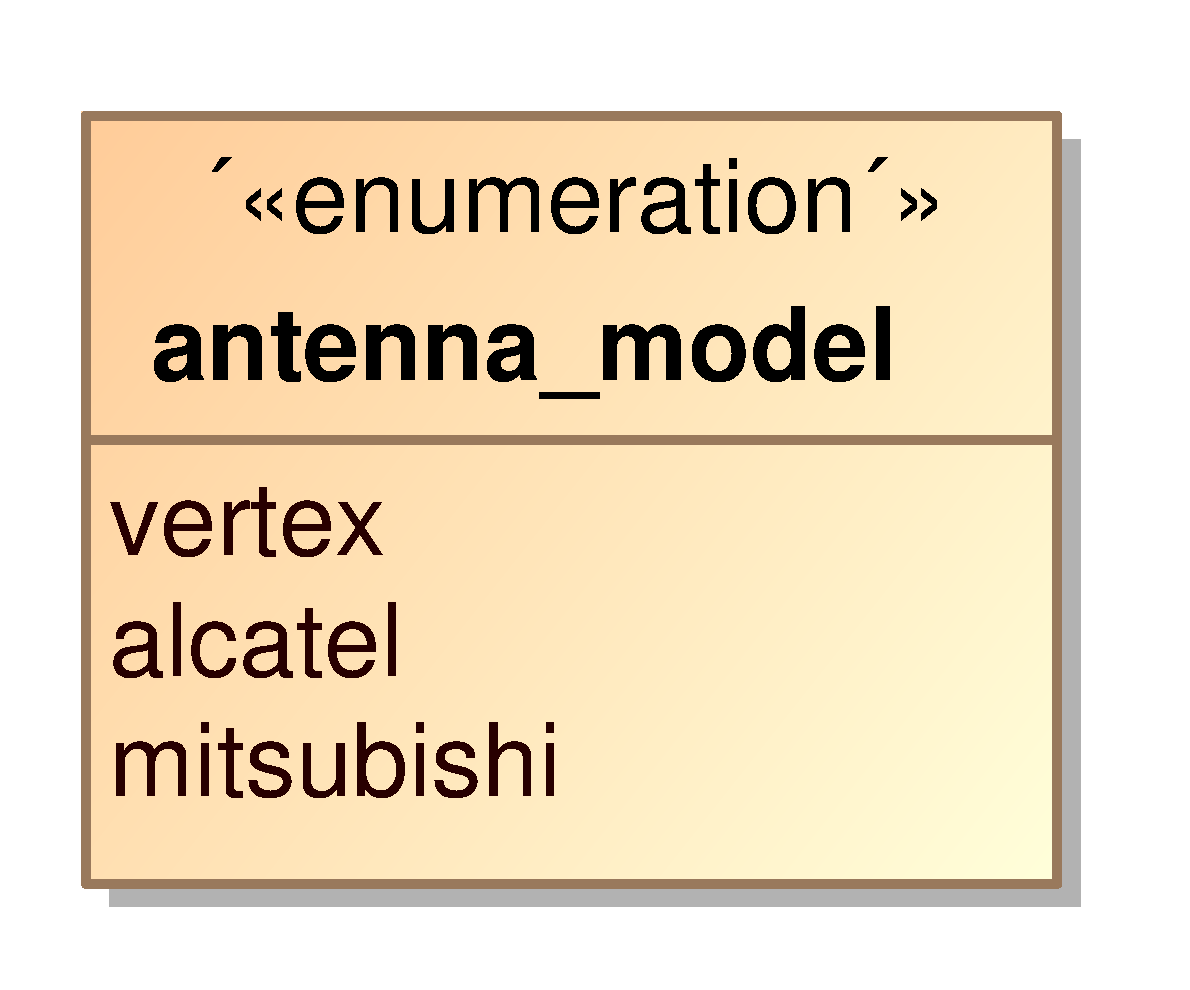
\includegraphics[scale=0.2]{images/enumeration}
\caption{\label{fig:vs_diag}Basic Enumeration Definition}
\end{center}
\end{figure*} 

An example of the code generated:

\begin{center}
\begin{verbatim}
....
module example3
{
    enum antenna_model { vertex, alcatel, mitsubishi };
....
\end{verbatim}
\end{center}

\subsubsection{Code Generated}

For convention, the model name has to be in a reverse domain name syntax,
(see the examples) i.e.:
\begin{center}
\begin{verbatim}
cl.alma.acsccg.example1
\end{verbatim}
\end{center}
The generator will generate the source code using the reverse domain name
syntax for generate the Java code. An example of the code generated for the
Figure 5 with the model name as \verb+cl.alma.acsccg.example1+ (this can be viewed in the folder structure).
\begin{center}
\begin{verbatim}
example3/
|-- idl
|   |-- BasicAntennaBase.idl
|   `-- example1Common.idl
|-- src
|   |-- cl
|   |   `-- alma
|   |       `-- acsccg
|   |           `-- example1
|   |               |-- BasicAntennaBaseHelper.java
|   |               `-- BasicAntennaBase.java
|   `-- Makefile
`-- test
    `-- CDB
        `-- MACI
            |-- Components
            |   `-- Components.xml
            |-- Containers
            	|-- javaContainer
            |   |   `-- javaContainer.xml
            |   `-- frodoContainer
            |       `-- frodoContainer.xml
            `-- Managers
                `-- Manager
                    `-- Manager.xml
\end{verbatim}
\end{center}

Also is generated the project Makefile, in which is defined the name of
the Jar file and the IDL interfaces to compile. The name of the Jar file is the last
name in the model name.

\newpage

\subsection{Java Interfaces}
The generator was designed to support Java interfaces in the UML model, this
interfaces are implemented by the generator writing the methods in the
component generated code.\\ 
\begin{figure*}[h!t]
\begin{center}
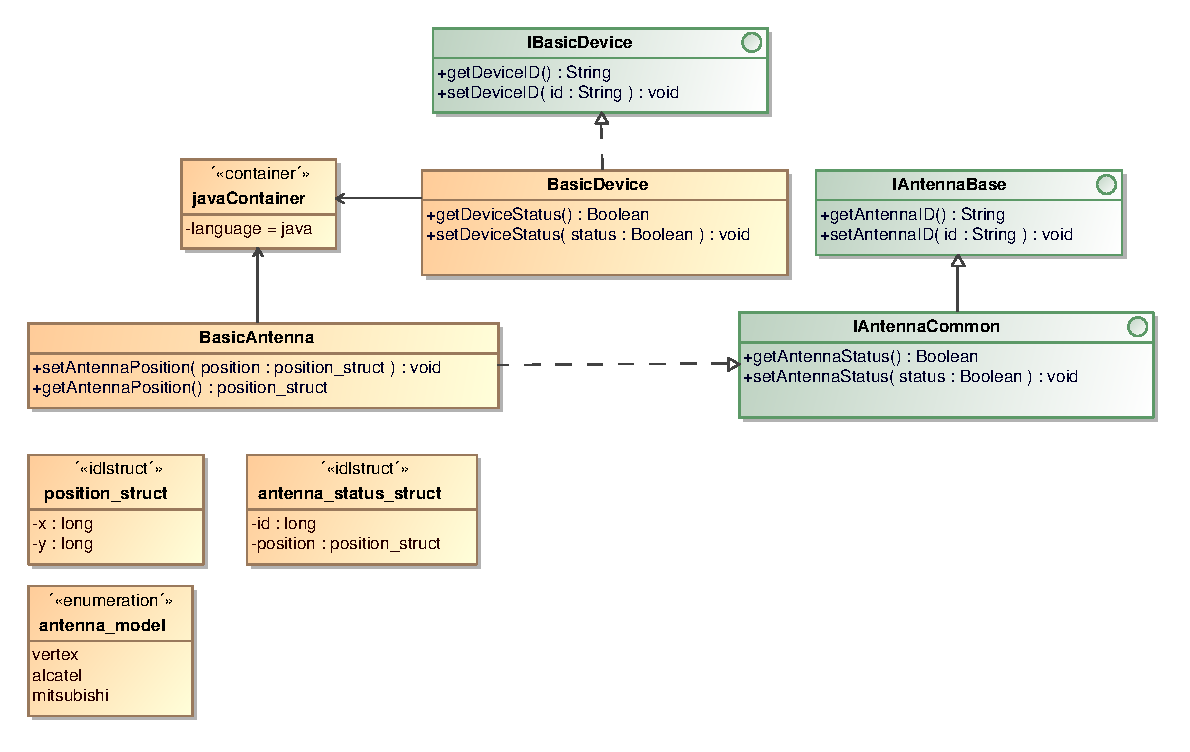
\includegraphics[scale=0.8]{images/example3}
\caption{\label{fig:vs_diag}Interfaces.}
\end{center}
\end{figure*}
\\
In the figure above, the class  \verb+BasicAntenna+ implements the Interface
\verb+IAntennaCommon+ and \verb+IAntennaCommon+ is extended from
\verb+IAntennaBase+, the generator also can implement the inheritance in
Interfaces. The code generated for the \verb+BasicAntenna+ component implements
the all the methods of all  implemented interfaces, if the interface is extended
in one or multiple levels, the generator implements all methods of the interface
inheritance (Java OOP constraints) and the IDL file implement this methods to.

Code generated, the component implementes the java interface defined in the
model above.
\begin{center}
\begin{verbatim}
...
public class BasicAntennaBase
      implements
         ComponentLifecycle,
              BasicAntennaBaseOperations,
              IAntennaCommon {
...
\end{verbatim}
\end{center}

And all methods from \verb+IAntennaCommon+, \verb+IAntennaBase+  are implemented
in the component.
\begin{center}
\begin{verbatim}
...
    /*
     * Implements the Interface methods.
     */
    @Override
    public boolean getAntennaStatus() {...

    @Override
    public void setAntennaStatus(boolean status) {...

    @Override
    public String getAntennaID() {...

    @Override
    public void setAntennaID(String id) {....
 ...
\end{verbatim}
\end{center}

Also the IDL file of the component is implemented with this methods to:
\begin{center}
\begin{verbatim}
...
#ifndef BasicAntenna_IDL
#define BasicAntenna_IDL
#include <acscomponent.idl>
#include <example3Common.idl>

#pragma prefix "alma"

module example3
{
    interface BasicAntennaBase : ACS::ACSComponent
    {
        void setAntennaPosition(in position_struct position);
        position_struct getAntennaPosition();
        boolean getAntennaStatus();
        void setAntennaStatus(in boolean status);
        string getAntennaID();
        void setAntennaID(in string id);
    };
};
#endif /* example3_IDL */
...
\end{verbatim}
\end{center}

This example can be downloaded from:
http://acsccg.googlecode.com/files/example3.tar.gz

\subsection{Inheritance}

\subsubsection{Multiple Level}
The generator is designed to support inheritance in one ore more inherited
levels, with the ability to override the inherited methods from the parenet, or,
override all methods inherited in all inherited levels.\\
This can be viewed in figure 11.

\begin{figure*}[h!t]
\begin{center}
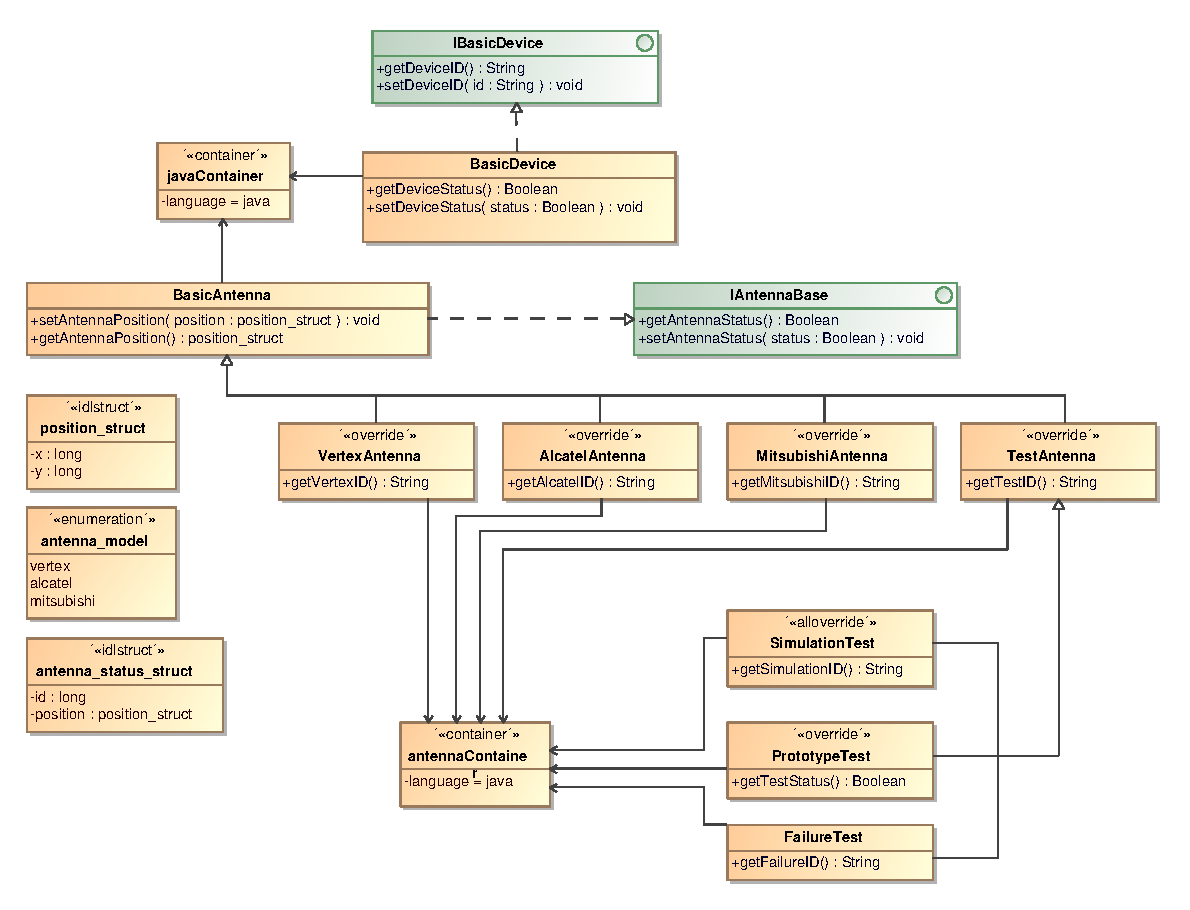
\includegraphics[scale=0.88]{images/example4}
\caption{\label{fig:vs_diag}Inheritance in the generator}
\end{center}
\end{figure*}

This example can be downloaded from:
http://acsccg.googlecode.com/files/example4.tar.gz

In the example above the classes with the  \verb+<<override>>+ stereotype will
override the methods from his parents in the Java generated code, and the
classes with the  \verb+<<alloverride>>+ will override all methods inherited in all
leves, i.e.: the class  \verb+SimulationTest+ will have his own methods, the 
\verb+TestAntenna+ methods, the  \verb+BasicAntenna+ methods (with the methods
of the implemented interface  \verb+IAntennaBase+).\\
If the component class has a parent class, the  \verb+initialize+ method of the
component will call the  \verb+initialize+ method of the parent class, an
example of this is:
\begin{center}
\begin{verbatim}
...
public class VertexAntennaBase extends BasicAntennaBase...

public void initialize(ContainerServices containerServices) {

		m_containerServices = containerServices;

		super.initialize(containerServices);
...
\end{verbatim}
\end{center}
The IDL files also implement the inheritance, an example of this:
\begin{center}
\begin{verbatim}
...
module example4
{
     interface AlcatelAntennaBase : BasicAntennaBase  
    {
        string getAlcatelID();
        void setAntennaPosition(in position_struct position);
        position_struct getAntennaPosition();
...
\end{verbatim}
\end{center}

Also if the class component is not inherited from other component or other
class, the IDL interface is extended from \verb+ACS::ACSComponent+, the
AlcatelAntennaBase is extended from BasicAntennaBase.

\subsection{Characteristic Component}
A class with the stereotype \verb+<<Characteristic>>+, if is extended from
other class, the generator will not implement the inheritance in the Java code,
because the Java OOP paradigm not support multiple inheritance (parallel
inheritance) and the class with \verb+<<Characteristic>>+, the generator will
generate the class already extended from ACS class
`CharacteristicComponentImpl`, also is generated the schema configuration .

\subsection{Notification Channel} 
 
 The ACS Notification Channel also is supported in the UML model.
 
 \begin{figure*}[h!t]
\begin{center}
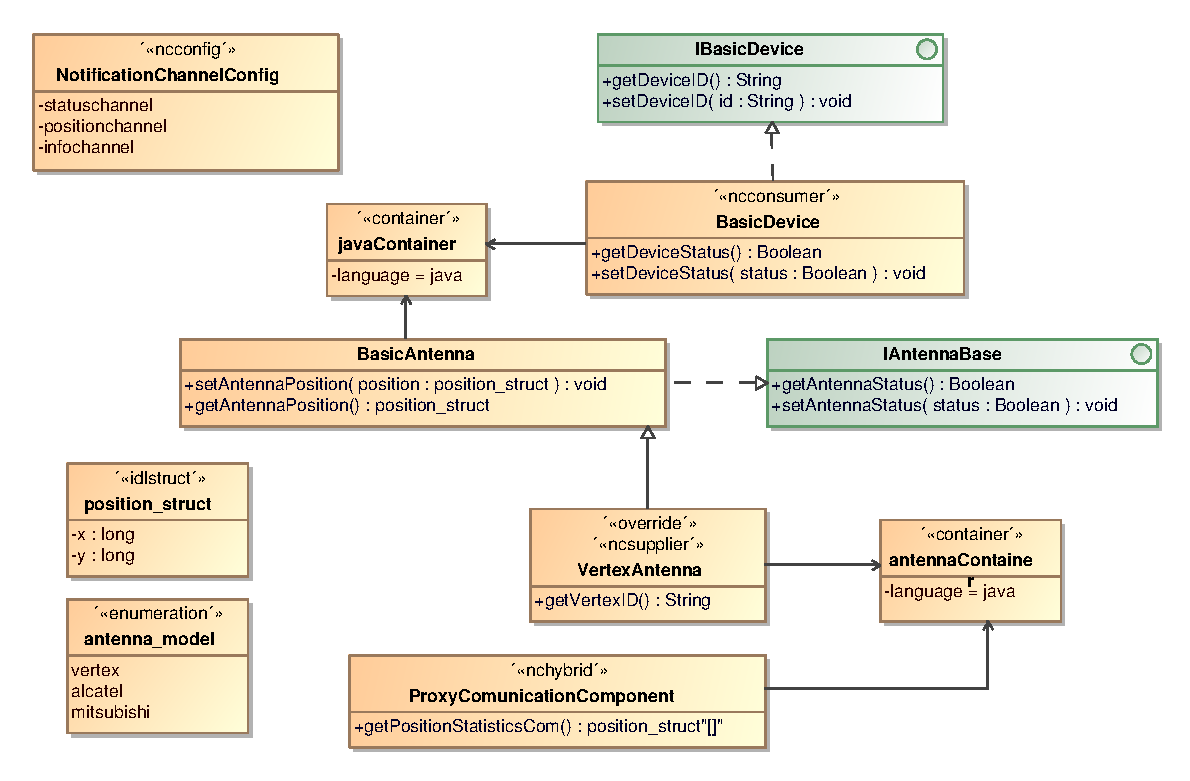
\includegraphics[scale=0.88]{images/example6}
\caption{\label{fig:vs_diag}Inheritance in the generator}
\end{center}
\end{figure*}
 
This example can be downloaded from:
http://acsccg.googlecode.com/files/example6.tar.gz\\
\\
In the example above exists a class with the \verb+<<ncconfig>>+ stereotype,
this class define the channels to use in the project, in the example they are
defined three channels \verb+statuschannel+, \verb+positionchannel+ and
\verb+infochannel+ generated in the common IDL interface, in this case
\verb+example6Common.idl+ , should only be one class with this stereotype.
\\
Also when this class is defined in the model, the generator define a common or
default channel called in this case \verb+defaultexample6channel+, the
\verb+example6+ in the channel name, is from the reverse domain name syntax on
model naming and a IDL struct for test the channel implementation, this struct
is called \verb+testMessageBlockEvent+, an example of the code generated :

\begin{center}
\begin{verbatim}
...
//Channels
const string CHANNELNAME_DEFAULTEXAMPLE6CHANNEL = "defaultexample6channel";
const string CHANNELNAME_STATUSCHANNEL = "statuschannel";
const string CHANNELNAME_POSITIONCHANNEL = "positionchannel";
const string CHANNELNAME_INFOCHANNEL = "infochannel";

 //Test Struct Event for the notification channels
struct testMessageBlockEvent
{
     double randomID;  
     string message;
 };
  typedef sequence<testMessageBlockEvent> testMessageBlockEvent_seq;
...
\end{verbatim}
\end{center}

Also in the example, they are classes with the \verb+<<ncsupplier>>+,
\verb+<<ncconsumer>>+ and the \verb+<<nchybrid>>+:

\subsubsection{ncsupplier}
The classes with  \verb+<<ncsupplier>>+ stereotype, will supply events in the
default channel defined by the generator, in this case the channel is called:\\
\verb+const string CHANNELNAME_DEFAULTEXAMPLE6CHANNEL="defaultexample6channel";+
Also the generator will implement the necessary methods to supply events ( a
default event called \verb+testMessageBlockEvent+) in the channel, an
example of the code generated:

\begin{center}
\begin{verbatim}
...

import alma.acs.nc.SimpleSupplier;
import alma.example6.testMessageBlockEvent;

...

    public void initialize(ContainerServices containerServices) {

        m_containerServices = containerServices;

        super.initialize(containerServices);

        m_logger = m_containerServices.getLogger();
        m_logger.info("initialize() called...");

        try {
            // Instantiate our supplier
                m_supplier = new SimpleSupplier(
                    alma.example6.CHANNELNAME_DEFAULTEXAMPLE6CHANNEL.value,
                m_containerServices);
        } catch (Exception e) {
            //throw new ComponentLifecycleException("failed to create
        SimpleSupplier for channel " + 
        alma.example6.CHANNELNAME_DEFAULTEXAMPLE6CHANNEL.value, e); 
        }

....

    public void sendEvents() throws CouldntPerformActionEx {
       m_logger.info("Now sending  testMessageBlockEvent events...");
        try {
            testMessageBlockEvent event = new testMessageBlockEvent(Math
                .random(), "Event");
            m_supplier.publishEvent(event);
        } catch (Throwable thr) {
            m_logger
                .log(Level.WARNING,
                    "failed to send testMessageBlockEvent. Will not try
                    again."); throw (new AcsJCouldntPerformActionEx(thr))
                    .toCouldntPerformActionEx();
        }
    }
\end{verbatim}
\end{center}

\subsubsection{ncconsumer}
The classes with  \verb+<<ncconsumer>>+ stereotype, will consume events in the
default channel defined by the generator, in this case the channel is called:\\
\verb+const string CHANNELNAME_DEFAULTEXAMPLE6CHANNEL="defaultexample6channel";+
Also the generator will implement the necessary methods to consume events ( a
default event called \verb+testMessageBlockEvent+) in the channel, an
example of the code generated:

\begin{center}
\begin{verbatim}
...
    private Consumer m_consumer;
    ....
        try {
            m_consumer = new Consumer(
                alma.example6.CHANNELNAME_DEFAULTEXAMPLE6CHANNEL.value,
                    m_containerServices);
                //Subscribe to a domain and event type.
            m_consumer.addSubscription(
                alma.example6.testMessageBlockEvent.class, this);
                m_consumer.consumerReady();
                m_logger
                    .info(" BasicDevice  is waiting for 
                    'testMessageBlockEvent'events."); 
                    } catch (Exception e) {
                if (m_consumer != null) {
            m_consumer.disconnect();
			           }
            /*
             if uncomment the next line, add  throws
             ComponentLifecycleException, but first check if is 
             inhitered class, can not be override the method. 
             the generator put the right code. */ 
             throw new ComponentLifecycleException( 
             "failed to connect as an event consumer to channel " +
             alma.example6.CHANNELNAME_DEFAULTEXAMPLE6CHANNEL.value); 
             }
    ....
    
...
\end{verbatim}
\end{center}


\subsubsection {nchybrid}
The classes with  \verb+<<nchybrid>>+ will consume and supply events in the
default channel defined by the generator, this class will implement the supply
and consume methods, variables and librarys to test the component. This methods
and variables are the same of the examples above.\\
\\
For the three stereotypes, if the components has not a parent class, the
generator will implement an ACS throw exception in the   \verb+initialize+
method of the component.

%\subsubsection{Abstract Classes}
%Same as interface implementation, the generator support the abstract class
%definition and generate the code.\\
%Classes with the \verb+<<Characteristic>>+ stereotype, the generator will no
%generate this classes as Abstract.

\subsection{Implemented Code vs Generated Code}
In every model driven development and code generators, is important how make a
strategy to separate the code already generated with the code implemented over
the generated code.\\
They are three ways solve this.

\subsubsection{EMF Veto Strategy and Inheritance}
The Veto EMF strategy (see Generator Optimization section) is a good solution
using inheritance to implement new things, but, must be create a new class for every change in our code to void
override the whole code already generated, so, this is not the best solution,
but, it works.

\subsubsection{GAP Desing Pattern}
The generation GAP desing pattern provides separate the code with all
hand-modifications implemented in sub-classes, this mean that the core classes
are generated only once and the hand-made implementations, are extended as
subclases from core classes.

\subsubsection{Protected Areas}
Xpand, provides protected areas to our generated code, this mean, that certain
areas with the protected tag with a unique autegenerated ID, can be modified by
the developer without loosing the hand-modifications over the generated code
when the code is re-generated (even if classes are changed in the model).
i.e.: This code went generated with protected areas.
\begin{verbatim}
1. public void getSimulationList() {
2. /*PROTECTED REGION ID(getSimulationList) ENABLED START*/
3.    //Implementation Method here!
4. /*PROTECTED REGION END*/
5. }

1. Method definition
2. Start Protected Area
3. Method hand implementation
4. End Protected Area
\end{verbatim}
Protected areas are specified in generator templates, the generator analize the
generated code, check the code with the template, and protect the area from the
regeneration. If the protected region is not in the templates, the generator
will void the area.\\
In methods, only the implementation is protected and for the code that scape
from UML model every class has a protected area for custom imports, variables and methods.

\section{HOW TO USE}

The usage of the code generator is pretty simple:

\begin{itemize}
\item Since the generator was designed to work better with MagicDraw models,
first create the model with the stereotypes defined in this document, a template
MagicDraw file can be downloded from:\\
http://acsccg.googlecode.com/files/TemplateModelMagicDraw.tar.gz .
\item It is recommended to create a folder with 3 subfolders inside, a
`generated` folder, a `model` folder and a `xmi` folder in which goes the
exported XMI files from MagicDraw.
\item Once the model is defined export the model in : `Eclipse UML2 (v2.x) XMI
FILE` export menu in MagicDraw.
\item Download the Jar Binary from:\\
http://acsccg.googlecode.com/files/ACSCCG.jar
\item Run the generator specifying the model path exported, profile file path
exported and the code path for the code generated:\\ 
\verb+java -jar acsComponentCodeGenerator.jar -model /my/very/path/to/MyProject.uml+ \\
\verb+-profile /my/very/path/to/Alma.profile.uml -output+\\
\verb+/user/home/MyProject/generated/folder+\\
\item In the project code page, they are 6 examples of models, image models,
XMI, generated code (tested), ready to download and run, each example represents
a feature of the generator.
\item Update the make file, see the `Knowing Problems` section in this document.
\end{itemize}

\subsection {Generator Command line Help} 
\begin{verbatim}
[atejeda@backorg Desktop]$ java -jar acsComponentCodeGenerator.jar 

ACSCodeGenerator
Compilation 100615

http://code.google.com/p/acsccg/
- Alexis Tejeda <alexis.tejeda@gmail.com>
- Nicolas Troncoso <ntroncos@alma.cl>

usage: java -jar acsComponentCodeGenerator.jar -model /my/very/path/to/MyProject.uml -profile
            /my/very/path/to/Alma.profile.uml -output
            /user/home/MyProject/generated/folder [options]
 -a              About this application
 -c <arg>    True if want to clean the output folder.. ! BEWARE ! will
            erase all from folder an parent folder !
 -h              Print help for this application
 -m <arg>   Model file path, i.e.: /my/very/path/to/MyProject.uml
 -o <arg>   The data source to use
 -p <arg>     Profile UML path, i.e.:
            /my/very/path/to/AlmaGenerator.profile.uml

 An Error has been found, see the help...
                                run: java -jar acsComponentCodeGenerator.jar -h

\end{verbatim}

\subsection {Keep eye on this} 
The generator has an option to clean the directory, this option by default is
disabled, because the output folder can be deleted manually, in case that if
this option is enabled, the generator will delete the destination folder and the
parent folder for the code generated, beware with the paths in case of enable
this option, can cause several damages.

\subsection {Constraints} 
\begin{itemize}
  \item The generator has been tested only with MagicDraw models, but can work
  with other XMI2.x UML models to.
  \item In the model, can exist only one package.
  \item The name of the model has to be in reverse domain name sintax (see the
  examples).
\end{itemize}

\newpage
\section{KNOWING PROBLEMS}

Since theres no order when the generator reads the model, must fix the IDL
compiling order in the Makefile following the the inheritance order,
i.e.: first compile the BasicAntenna, then compile the VertexAntenna IDL
(VertextAntenna is extended from BasicAntenna) files.\\
\\
The common IDL file wich have common structs, channel names..etc... many
structs have other structs data types, for fix this, just reorder the structs in the
common IDL file.

\section{FUTURE WORK AND WHAT IS NEXT}

\subsection {Future work}
\begin{itemize}
  \item Specify the channel and events that a component would use.
  \item Add custom documentation in the methods and class through the UML model.
  \item Package implementation in the same model.
\end{itemize} 

\subsection {What is next}
In discussion\ldots
\newpage
\section{PROJECT SITES}

Jao Twiki page:
\begin{itemize}
	\item http://almasw.hq.eso.org/almasw/bin/view/JAO/ACSCodeGenerationReports
	\item http://almasw.hq.eso.org/almasw/bin/view/Main/AlexisTejedaDailyWorklog
	\item http://almasw.hq.eso.org/almasw/bin/view/JAO/ACSCodeGeneration
\end{itemize}

Project code:
\begin{itemize}
	\item Main site: http://code.google.com/p/acsccg/
	\item Binarys and Downloads: http://code.google.com/p/acsccg/downloads/list
	\item Issues report: http://code.google.com/p/acsccg/issues/list
	\item Source : http://code.google.com/p/acsccg/source/checkout
\end{itemize}
 
 Source Trunk and Branches:
 \begin{itemize}
	\item Development: https://acsccg.googlecode.com/svn/branches/acsccg-devel
	\item Documentation: https://acsccg.googlecode.com/svn/branches/acsccg-doc
	\item Examples:  https://acsccg.googlecode.com/svn/branches/acsccg-examples
	\item Trunk: https://acsccg.googlecode.com/svn/trunk/
\end{itemize}

The last stable release is always in the trunk, the nighty builds in the
Development branch, and the latest stable but not tested in Tags.\\
\\To browse thesource code:
\\
http://code.google.com/p/acsccg/source/browse/
\\

More info about the generator, doubts, etc, feel free to send a email to:\\
\verb+A.TEJEDA <alexis.tejeda@gmail.com>+




%% LAST PAGE AND DOCUMENT END
%\newpage
%\vspace*{10cm}
%\begin{figure*}[h!t]
%\begin{center}
%\includegraphics*[scale=2.2]{images/end-symbol.eps}
%\end{center}
%\end{figure*}

\end{document}
